\documentclass{_mypackages/monograph}

\title{Astrophysics} % \MyTitle
\author{Bruno Murino} % \MyAuthor
\date{\today} % \MyDate

\addbibresource{cosmology.bib}
\graphicspath{ {figures/} }

\begin{document}
\frontmatter

\monographtp
\dominitoc
\doparttoc
\pagestyle{onlypagenum}
\tableofcontents
\mainmatter

\chapter{Introduction}

\section{Luminosity}

\begin{definition}[Luminosity]
The amount of electromagnetic energy a body radiates in all directions per unit of time is called the body's \emph{luminosity} and varies with the wavelength observed. If \(L\) denotes the luminosity, then \([L] = \si{\watt} = \si{\joule\per\second}\).
\end{definition}

Let \(S\) be the luminosity flux we measured, in \si{\watt\per\metre\squared}, for a nearby galaxy, for which redshift corrections can be neglected. Then the luminosity of the galaxy is \(L = 4\pi r^2 S\), in \si{\watt}, where \(r\) is the distance of the galaxy.

\begin{definition}[Space density]
The frequency of occurrence per specified volume of space.
\end{definition}

\begin{definition}[Luminosity function]
The luminosity function of galaxies \(\phi(L)\dd{L}\) is defined to be the space density of galaxies with intrinsic luminosities in the range \(L\) to \(L + \dd{L}\), i.e. the amount of galaxies with luminosities in the range \(L\) to \(L + \dd{L}\) on a given volume of space.
\end{definition}

After some experiments, it was shown that function proposed by Schechter\footnote{Paul Schechter (May 30, 1948 -).}, i.e. Schechter function, is the one that best fits the collected data.

\begin{definition}[Schechter function]
The function defined by
\begin{equation}
    \phi(x)\dd{x} = \phi^* x^\alpha \exp{-x}\dd{x}
\end{equation}
is called the \emph{Schechter function}.
\end{definition}

\subsection{Photometry}

\begin{definition}[Passband \emph{or} filter]
The range of frequencies or wavelengths that can pass through a filter with minimum loss is called the \emph{passband}. 
\end{definition}

Of course, if different filters are used, different measurement's outputs are expect. So in order to allow accurate comparison between observations we need to classify the filters, and we do so by specifying which wavelength passes through the filter with the lowest loss, i.e. the \emph{effective wavelength midpoint for standard filters} and the \emph{full width half maximum}. The most common filters have special names and properties. See \href{https://en.wikipedia.org/wiki/Photometric_system#Filters_used}{Photometric system}.

Lets get back to measuring the luminosity.

The light emitted from the surface of a celestial object must travel across some portion of the universe so it can reach us, and then, be measured by us. However, since there's not only vacuum between a celestial object and us, some fraction of the original light is lost, thus the only thing we can measure is this deprecated light, i.e. deprecated luminosity flux. But before we go on, lets introduce the concept of \emph{magnitude}, first proposed by Hipparchus\footnote{Hipparkhos Nikealainen (c.190 – c.120 bc), greek.} or Ptolemy\footnote{Claudius Ptolemaeus (AD 100 – c.170), greco-roman.} about 2000 years ago, but which modern definition we owe to N. Pogson\footnote{Norman Robert Pogson (23 March 1829 – 23 June 1891), english astronomer}. 

Pogson's idea was to create a scale such that, to each factor of \(100\) on the luminosity measured, the new unit called \emph{magnitude} should decrease by \(5\), i.e. a scale following \emph{Pogson's ratio}: \(\sqrt[5]{100} = 2.512\).

\begin{definition}[Magnitude]
Lets suppose we do a measurement of luminosity with the filter \(x\). Let \(S_{x,0}\) be the reference flux for the filter \(x\) and \(S_x\) the flux we measured. Then \(m_x\) defined by
\begin{equation}
    m_x = - 5 \log_{100}\left(\frac{S_x}{S_{x,0}} \right) = - 2.5 \log_{10}\left(\frac{S_x}{S_{x,0}} \right)
\end{equation}
is called the \emph{magnitude} of the celestial object.
\end{definition}

Since this measurement depends on the distance we are from the celestial object, its not an intrinsic property of it.

\begin{definition}[Apparent magnitude]
If the measurement is performed from the Earth, then the magnitude measured is called the \emph{apparent magnitude}.
\end{definition}

\begin{definition}[Absolute magnitude]
If the measurement could be taken exactly \SI{10}{\parsec} away from the celestial body, the magnitude measured would be the \emph{absolute magnitude}. In other words, the absolute magnitude is defined as what we would measure if the measurement could take place exactly \SI{10}{\parsec} away from the celestial body.
\end{definition}

Its not absurd to think that luminosities should obey the inverse square law, i.e. the apparent magnitude should increase by a factor of 4 if the distance increases by a factor of 2. First, lets define the distance modulus.

\begin{definition}[Distance modulus]
The difference \(\mu = m - M\), where \(m\) is the apparent magnitude and \(M\) is the absolute magnitude, is called the \emph{distance modulus}.
\end{definition}

\begin{definition}[Luminosity distance]
A distance obtained by means of luminosities is called a \emph{luminosity distance}.
\end{definition}

\begin{mybox}
Bearing in mind the inverse square law, we can write the following relation between the distance modulus and the luminosity distance:
\begin{equation}\label{eq:magdis}
    \mu = m - M = 5 \log_{10} \left( \frac{d}{\SI{10}{\parsec}}\right)
\end{equation}
where \(\mu\) is the distance modulus, \(m\) is the apparent magnitude, \(M\) is the absolute magnitude and \(d\) is the luminosity distance.
\end{mybox}



\subsection{Velocity dispersion}

Galaxies are composed of stars and some other objects, and all this objects are moving with some velocity.

\begin{definition}[Velocity dispersion]
If we measure the velocity of the stars of a galaxy and plot the results in a histogram we will find the stars' velocity distribution. The standard deviation of this velocity distribution is called the \emph{velocity dispersion}.
\end{definition}

\begin{definition}[Central velocity dispersion]
Let \(G\) be a galaxy composed of stars \(s\in G\). If we measure the velocity distribution of stars only near the centre of the galaxy and then compute its velocity dispersion, the result we find will be the so called \emph{central velocity dispersion}.
\end{definition}

\subsection{Don't know}

\begin{definition}[Surface brightness]
The surface brightness is defined as the photon energy received by a unit area at the observer per unit time from a unit solid angle in a specific direction.
\end{definition}

\begin{definition}[Isophotes]
The contours along which the surface brightness of a source is constant are called \emph{isophotes}.
\end{definition}

\begin{notation}
The isophotal curve of magnitude \(n\) is denoted \(Vn\).
A typical limit is 25 mag arcsec2.
\end{notation}

\begin{definition}[Stellar mass]
The mass of a star is often called the \emph{stellar mass}.
\end{definition}


\section{Elliptical galaxies}

\subsection{The Faber-Jackson Relation} 
Faber\footnote{Sandra Moore Faber (December 28, 1944 - ).} and Jackson\footnote{Robert Earl Jackson (1949 - ).}, in 1976\footfullcite{1976ApJ...204..668F}, noticed that the luminosity of an elliptical galaxy is correlated with its central velocity dispersion:
\begin{equation}
    L \propto \sigma_0^\beta \qq{with} beta \sim 4
\end{equation}

Thus if the apparent luminosity of two galaxies with the same central velocity dispersion is given, we can find the ratio between their distance.

\begin{figure}
    \centering
    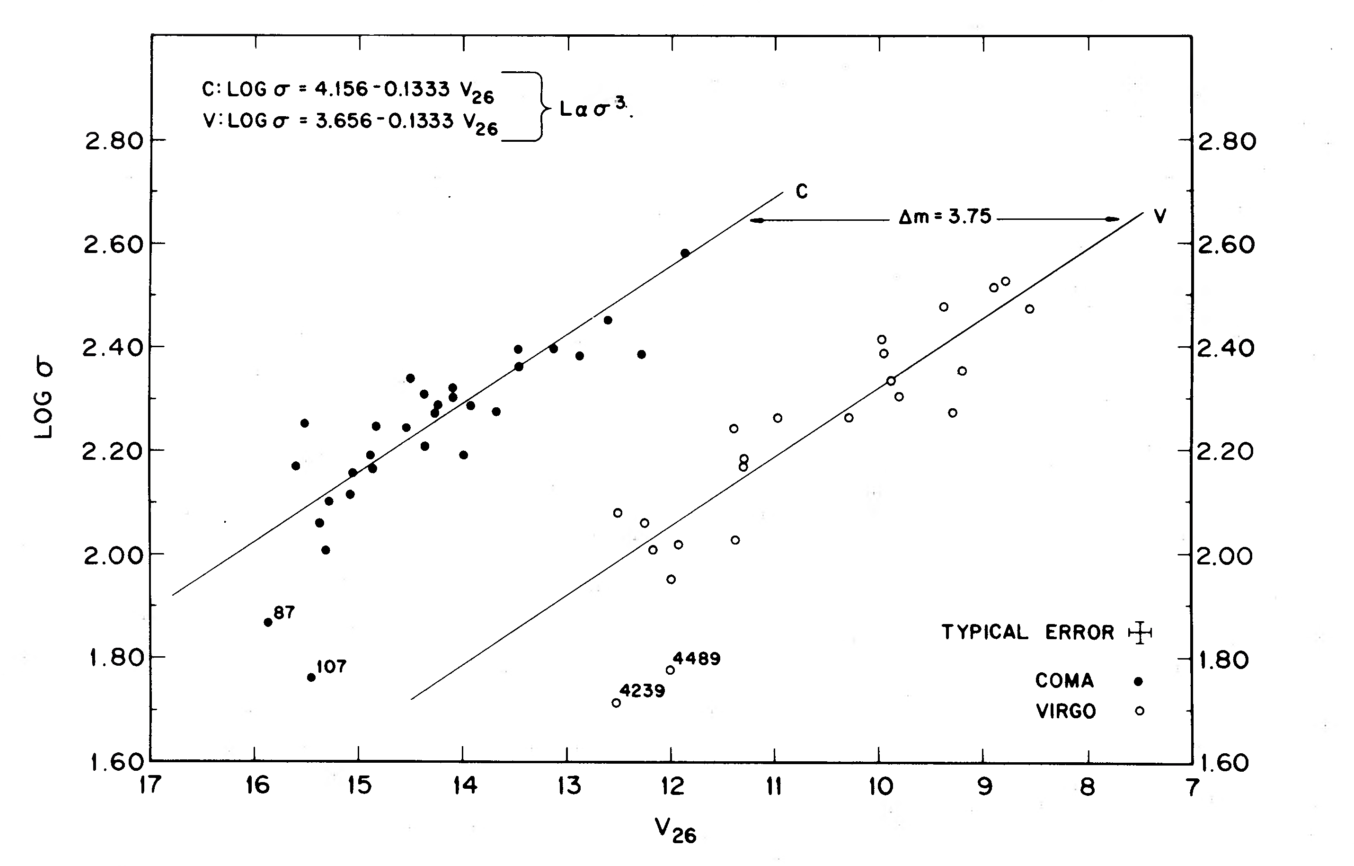
\includegraphics[width=\textwidth]{Astrophysics/figures/faber-jackson.png}
    \caption{The log of the velocity dispersion vs. V26 for the Coma and Virgo ellipticals. The lines represent median fits, as described in the text, and are separated by 3.75 mag, indicating a distance ratio D(Coma)/D(Virgo) = 5.62. This implies a peculiar Virgocentric velocity of 311 km s-1. Some of the more deviant points are identified. (from \cite{Dressler1984}).}
    \label{fig:faber-jackson}
\end{figure}

From figure \ref{fig:faber-jackson} we can compare the apparent magnitude of the Virgo and Coma clusters when their central velocity dispersion is the same and find it to be around \(\num{3.75}\).

Now, taking equation \eqref{eq:magdis} for both clusters we find
\begin{gather}
    m_V - M_V = 5 \log_{10} \left( \frac{d_V}{\SI{10}{\parsec}}\right) \\
    m_C - M_C = 5 \log_{10} \left( \frac{d_C}{\SI{10}{\parsec}}\right)
\end{gather}
Since we will read the apparent magnitudes from \ref{fig:faber-jackson} when their central velocity distribution is the same, their absolute magnitude will be the same, thus subtracting one equation from the other we find
\begin{equation}
    m_V - m_C - (M_V - M_C) = m_V - m_C = 5 \log_{10} \left( \frac{d_V}{d_C}\right)
\end{equation}
but since \(m_V - m_C = -3.75\), we find that \(\nicefrac{d_C}{d_V} = 5.62\), which means that the Virgo cluster is closer to us than the Coma cluster.

\chapter{Cosmology}
% \minitoc

\section{Redshift}

\subsection{The age of the universe at given redshift}

In the Einstein-de Sitter model of the universe:

\begin{equation}
    t(z) = \tau_H \int_{z}^{\infty} \frac{\dd{z}'}{(1+z')E(z')}
\end{equation}
where \(E(z) = (1+z)^{3/2}\), thus
\begin{equation}
    t(z) = \tau_H \int_{z}^{\infty} \frac{\dd{z}'}{(1+z')^{5/2}} =  \tau_H \frac{2 }{3(z+1)^{3/2}}
\end{equation}
with \(\tau_H =  H_0^{-1} = \SI{9.78 }{h^{-1} \giga\year}\).

For \(z=20\) and the accepted value of \(h=0.7\), then, the age of the universe is
\begin{equation}
    t(20) = \SI{9.78}{h^{-1} \giga\year}\, \frac{2}{3(21)^{3/2}} = \frac{6.52}{0.7*96.2341} = \SI{0.097}{\giga\year} = \SI{97}{\mega\year}
\end{equation}


\subsubsection{Roche radius}

Consider a satellite orbiting a \emph{primary body}. The primary exerts a tidal force on the satellite, i.e. the patch of the satellite closest to the primary feels a bigger gravitational pull than the rest of the satellite. 

For computation purposes, let's denote this closest patch by a mass \(\mu\), and let's denote the rest of the satellite by a mass \(m\), which we'll consider to be centred on the satellite. Then, regarding only the action of the primary on the satellite, the relative force experienced by \(\mu\) at different distances the so called \emph{tidal force}. We also have to consider the mutual attraction between \(\mu\) and \(m\), however, assuming \(\mu \ll m\), the force \(m\) experiences due to \(\mu\) is negligible.

The tidal force can be written as
\begin{equation}
    F_T = \frac{GMu}{(d-r)^2} - \frac{GMu}{d^2} \approx \frac{2GMu r}{d^3},
\end{equation}
while the usual gravitational force of the bigger part of the satellite over the small part can be written as
\begin{equation}
    F_G = \frac{Gmu}{r^2}.
\end{equation}

We want to find at what distance from the primary the satellite the tidal force will be bigger than the \(F_G\):
\begin{equation}
\begin{split}
    F_T &> F_G \\
    \frac{2GMu r}{d^3} &> \frac{Gmu}{r^2} \\
    2\frac{M}{m} r^3 &> d^3,
\end{split}
\end{equation}
which leads to
\begin{equation}
    d < r \left(\frac{2M}{m}\right)^{1/3},
\end{equation}
or
\begin{equation}
    d < R\left(\frac{2\rho_M}{\rho_m}\right)^{1/3}.
\end{equation}



\backmatter
\printbib
\end{document}
